\documentclass[aspectratio=169, 10pt]{beamer}
\usetheme{metropolis}

%%% Проверка используемого TeX-движка %%%
\usepackage{iftex}[2013/04/04]
\newif\ifxetexorluatex   % определяем новый условный оператор (http://tex.stackexchange.com/a/47579/79756)
\ifXeTeX
    \xetexorluatextrue
\else
    \ifLuaTeX
        \xetexorluatextrue
    \else
        \xetexorluatexfalse
    \fi
\fi

\RequirePackage{etoolbox}[2015/08/02]               % Для продвинутой проверки разных условий

%%% Поля и разметка страницы %%%

\usepackage{pdflscape}                              % Для включения альбомных страниц
\usepackage{geometry}                               % Для последующего задания полей

%%% Математические пакеты %%%
\usepackage{amsfonts,amsmath,amssymb,amscd,amsthm}  % Математические дополнения от AMS
% %amsthm should be loaded after amsmath!!

\usepackage{mathtools}                              % Добавляет окружение multlined

%%%% Установки для размера шрифта 14 pt %%%%
%% Формирование переменных и констант для сравнения (один раз для всех подключаемых файлов)%%
%% должно располагаться до вызова пакета fontspec или polyglossia, потому что они сбивают его работу
\newlength{\curtextsize}
\newlength{\bigtextsize}
\setlength{\bigtextsize}{13.9pt}

\makeatletter
%\show\f@size                                       % неплохо для отслеживания, но вызывает стопорение процесса, если документ компилируется без команды  -interaction=nonstopmode 
\setlength{\curtextsize}{\f@size pt}
\makeatother

% %%% Кодировки и шрифты %%%
% \ifxetexorluatex
%     \usepackage{polyglossia}[2014/05/21]            % Поддержка многоязычности (fontspec подгружается автоматически)
% \else
%     \RequirePDFTeX                                  % tests for PDFTEX use and throws an error if a different engine is being used
%    %%% Решение проблемы копирования текста в буфер кракозябрами
% %    \input glyphtounicode.tex
% %    \input glyphtounicode-cmr.tex %from pdfx package
% %    \pdfgentounicode=1
%     \usepackage{cmap}                               % Улучшенный поиск русских слов в полученном pdf-файле
%     \defaulthyphenchar=127                          % Если стоит до fontenc, то переносы не впишутся в выделяемый текст при копировании его в буфер обмена
    
% %    \usepackage[T2A]{fontenc}                       % Поддержка русских букв
%     \usepackage[T2A,T1]{fontenc}
%     \usepackage[utf8]{inputenc}[2014/04/30]         % Кодировка utf8
%     \usepackage[english, russian]{babel}[2014/03/24]% Языки: русский, английский
% \fi
% \usepackage{tempora} %TemporaLGCUni of Times type
% \usepackage{newtxmath} %math font of Times type
% % need to set the monospace=typewritter font
% %https://tex.stackexchange.com/questions/213835/using-many-typewriter-fonts-in-a-single-document
\usepackage{fontspec, lipsum}
\usepackage[utf8]{inputenc}
\usepackage[T1,T2A]{fontenc}
\usepackage{textcomp}
\usepackage[english, russian]{babel}

% Математические шрифты как в LaTeX
% \DeclareMathAlphabet{\mathcal}{OMS}{cmsy}{m}{n}
% \let\mathbb\relax % remove the definition by unicode-math
% \DeclareMathAlphabet{\mathbb}{U}{msb}{m}{n}

% % Шрифты документа (текст)
% \setmainfont[Ligatures=TeX]{CMU Serif} % обычный текст
\setmainfont[Ligatures=TeX]{Times New Roman} % обычный текст
% \setmonofont{Fira Code Regular} % код



\makeatletter %load fonts for cmtt
\providecommand{\EC@ttfamily}[5]{%
	\DeclareFontShape{#1}{#2}{#3}{#4}{
		<-8.5>#50800
		<8.5-9.5>#50900
		<9.5-10.5>#51000
		<10.5-11.5>#51095
		<11.5-13>#51200
		<13-15.5>#51440
		<15.5-18.5>#51728
		<18.5-22>#52074
		<22-27>#52488
		<27-32>#52986
		<32->#53583}{}}
\DeclareFontFamily{T1}{cmtt}{}
\DeclareFontFamily{T2A}{cmtt}{}
\EC@ttfamily{T1}{cmtt}{m}{n}{ectt}
\EC@ttfamily{T1}{cmtt}{m}{sl}{ecst}
\EC@ttfamily{T1}{cmtt}{m}{it}{ecit}
\EC@ttfamily{T1}{cmtt}{m}{sc}{ectc}
\DeclareFontShape{T1}{cmtt}{bx}{n}%
{<->ssub*cmtt/m/n}{}
\DeclareFontShape{T1}{cmtt}{bx}{it}%
{<->ssub*cmtt/m/it}{}
\EC@ttfamily{T2A}{cmtt}{m}{n}{latt}
\EC@ttfamily{T2A}{cmtt}{m}{sl}{last}
\EC@ttfamily{T2A}{cmtt}{m}{it}{lait}
\EC@ttfamily{T2A}{cmtt}{m}{sc}{latc}
\DeclareFontShape{T2A}{cmtt}{bx}{n}%
{<->ssub*cmtt/m/n}{}
\DeclareFontShape{T2A}{cmtt}{bx}{it}%
{<->ssub*cmtt/m/it}{}
\makeatletter

%\makeatletter %load fonts for cmtt
%\providecommand{\EC@ttfamily}[5]{%
%	\DeclareFontShape{#1}{#2}{#3}{#4}{
%		<-8.5>#50800
%		<8.5-9.5>#50900
%		<9.5-10.5>#51000
%		<10.5-11.5>#51095
%		<11.5-13>#51200
%		<13-15.5>#51440
%		<15.5-18.5>#51728
%		<18.5-22>#52074
%		<22-27>#52488
%		<27-32>#52986
%		<32->#53583}{}}
%\DeclareFontFamily{T2A}{cmtt}{\hyphenchar\font\m@ne}
%\EC@ttfamily{T2A}{cmtt}{m}{n}{latt}
%\EC@ttfamily{T2A}{cmtt}{m}{sl}{last}
%\EC@ttfamily{T2A}{cmtt}{m}{it}{lait}
%\EC@ttfamily{T2A}{cmtt}{m}{sc}{latc}
%\DeclareFontShape{T2A}{cmtt}{bx}{n}%
%{<->ssub*cmtt/m/n}{}
%\DeclareFontShape{T2A}{cmtt}{bx}{it}%
%{<->ssub*cmtt/m/it}{}
%\makeatletter

%\makeatletter
%\input{t1lmtt.fd}
%\@namedef{T1+lmtt}{}
%\makeatother


\renewcommand{\ttdefault}{cmtt}
%\renewcommand{\ttdefault}{lcmtt} %покрупнее
%\usepackage[scaled=.85]{DejaVuSansMono} %слишком похож на рубленый
%\newfont{\wasyten}{wasy10} %название команды для вызова / название шрифта



%Другие шрифты:
% математика
%\usepackage[lite]{mtpro2}
%https://pctex.com/mtpro2.html
% текст        
% https://www.ctan.org/pkg/paratype
%       \usepackage[scaled=0.925]{XCharter}[2017/06/25] % Подключение русифицированных шрифтов XCharter
%\usepackage{pscyr}
%    \IfFileExists{pscyr.sty}{}{}  % Красивые русские шрифты
%\fi

%https://tex.stackexchange.com/questions/8260/what-are-the-various-units-ex-em-in-pt-bp-dd-pc-expressed-in-mm
\usepackage{printlen} %для измерения и вывода параменторов шрифтов, отступов, интервалов

\usepackage{bm} %для жирных начертаний символов

\usepackage{csquotes} %to check quotes

%%% Оформление абзацев %%%
\usepackage{indentfirst}                            % Красная строка

%%% Цвета %%%
%\usepackage[dvipsnames,usenames]{color}
\usepackage{colortbl}
\usepackage[dvipsnames, table, hyperref, cmyk]{xcolor} % Вероятно, более новый вариант, вместо предыдущих двух строк. Конвертация всех цветов в cmyk заложена как удовлетворение возможного требования типографий. Возможно конвертирование и в rgb.

%%% Таблицы %%%
\usepackage{longtable}                              % Длинные таблицы
\usepackage{multirow,makecell}                      % Улучшенное форматирование таблиц:
													% multirow - строки на несколько ячеек, 
												
													% makecell - сесколько строк в ячейке.
													% не работает, если внутри, например, \verb|text| -> \texttt{text}
													% аналоги
%https://tex.stackexchange.com/questions/2441/how-to-add-a-forced-line-break-inside-a-table-cell								
						
													

%%% Общее форматирование
%\usepackage{soul} % используется ulem
\usepackage{soulutf8}                               % Поддержка переносоустойчивых подчёркиваний и зачёркиваний
\usepackage{icomma}                                 % Запятая в десятичных дробях



%%% Предметный указатель  ГОСТ 7.78-99 Index %%%
%c обобщенными рубриками или развернутый
%или указатель терминов (в общем случае - произвольное число указателей)
%подключать до hyperref

%\usepackage{makeidx} %возможно, необходимо подключить И/ИЛИ пройти Tools-> Commands -> MakeIndex

\usepackage{imakeidx} 
%\indexsetup{level=\section*,toclevel=section,noclearpage}
\makeindex[program=makeindex,
options=-s template_settings/common/myindex.ist, %подключаем стилевой файл для форматирования вывода
name=ru, % префикс для русских указателей 
% если убрать <<ru>>, то для работы дефолтового придется вручную включать Tools-> Commands -> MakeIndex
title={\chapterLight{} 
%   \hrule{}
	Предметный указатель
%	\hrule{}
} 
%,columns=1 %по умолчанию 2
]
\makeindex[program=makeindex,
options=-s template_settings/common/myindex.ist, %подключаем стилевой файл для форматирования вывода
name=en, % префикс для английских указателей
title={\chapterLight{}
%	\hrule{}
	Index
%	\hrule{}
} 
%,columns=1 %по умолчанию 2
] 
%убрать добавление <<title>> в содержание:
%\noindexintoc %not to add index title in PURE makeidx %intoc is false by default with imakeidx


%       https://tex.stackexchange.com/a/132415/44348
%\makeatletter
%% we want hyphenation also in the first word
\renewcommand{\@idxitem}{\par\hangindent40\p@\hspace{0pt}\ignorespaces}
%% we don't want a page break before a subitem %implemented in the previous one
%%\renewcommand\subitem{\@idxitem\nobreak\hspace*{20\p@}}
%\makeatother


%%% Фиксация плавающих объектов





%%% Гиперссылки %%%
\usepackage{hyperref}[2012/11/06]

%%% Изображения %%%
\usepackage{graphicx}[2014/04/25]                   % Подключаем пакет работы с графикой

%%% Списки %%%
\usepackage[shortlabels]{enumitem} % shortlabels для того, чтобы изменять токены в списках с дефолтных (иерархическая структура) на произвольныею

%%% Подписи %%%
\usepackage{caption}[2013/05/02]                    % Для управления подписями (рисунков и таблиц) % Может управлять номерами рисунков и таблиц с caption %Иногда может управлять заголовками в списках рисунков и таблиц


\usepackage{subcaption}[2013/02/03]                 % Работа с подрисунками и подобным

%%% Счётчики %%%
%\usepackage[figure,table]{totalcount}               % Счётчик рисунков и таблиц. Взамен используется xassoccnt 
\usepackage{totcount}                               % Пакет создания счётчиков на основе последнего номера подсчитываемого элемента (может требовать дважды компилировать документ)
\usepackage{totpages}                               % Счётчик страниц, совместимый с hyperref (ссылается на номер последней страницы). Желательно ставить последним пакетом в преамбуле

\usepackage{xassoccnt} % для подсчета сумм приложений, рисунков, таблиц 


%%% Продвинутое управление групповыми ссылками (пока только формулами) %%%
\ifxetexorluatex
    \usepackage{cleveref}                           % cleveref корректно считывает язык из настроек polyglossia
\else
    \usepackage[russian]{cleveref}                  % cleveref имеет сложности со считыванием языка из babel. Такое решение русификации вывода выбрано вместо определения в documentclass из опасности что-то лишнее передать во все остальные пакеты, включая библиографию.
\fi
\creflabelformat{equation}{#2#1#3}                  % Формат по умолчанию ставил круглые скобки вокруг каждого номера ссылки, теперь просто номера ссылок без какого-либо дополнительного оформления



\ifnumequal{\value{draft}}{1}{% Черновик
    \usepackage[firstpage]{draftwatermark}
    \SetWatermarkText{DRAFT}
    \SetWatermarkFontSize{14pt}
    \SetWatermarkScale{15}
    \SetWatermarkAngle{45}
}{}



\usepackage{tikz}
\usetikzlibrary{arrows,automata,positioning}
\usepackage{lastpage}

\usepackage{unicode-math}
% \setmainfont{FiraCode-Retina.ttf}
\setmathfont{mathFont.ttf}

\definecolor{notImportant}{HTML}{888888}
\definecolor{mathematicaBlue}{HTML}{ACBDD7}
\definecolor{mathematicaYellow}{HTML}{F9D391}

\newcommand{\notImportant}[1]{{\color{notImportant}\small{}#1}}

\newcommand{\jpExample}[2]{#1 \\ --- #2.}
\newcommand{\sourceSentence}[1]{\notImportant{(1) Исходное предложение: }\\ #1}
\newcommand{\transformerSample}[1]{\notImportant{(2) Изначальная модель (Transformer): }\\ #1}
\newcommand{\pretrainedTransformerSample}[1]{\notImportant{(3) Модифицированная модель (Pretrained Transformer): }\\ #1}

\begin{document}
  \nocite{*}
  % \setbeamertemplate{footline}{\insertframenumber/\inserttotalframenumber}
  % %!TeX root = ../SimplifyJapanese.tex
\begin{frame}[plain]{}
  \setbeamertemplate{section in toc}[sections numbered]
  % \tableofcontents[hideallsubsections]
  \begin{center}%
    \footnotesize
    Санкт-Петербургский политехнический университет Петра Великого \\ 
    Институт компьютерных наук и технологий \\ 
    Высшая школа интеллектуальных систем и суперкомпьютерных технологий
  \end{center}
  \vfill
  \begin{center}%
    Выпускная квалификационная работа магистра \\
    \Large
    \uppercase{Разработка и исследование системы автоматического упрощения текстов на японском языке} \\[6pt]
    \scriptsize
    Направление: \\
    «Математическое обеспечение и администрирование информационных систем»
  \end{center}
  \vfill
  \footnotesize
  \begin{tabularx}{\textwidth}{LcR}%
    Выполнил: &  &  Научный руководитель: \\ 
    студент гр.~3540203/00101 & Санкт-Петербург &  к.\,ф.--м.\,н., доцент ВШИИ \\
    \textbf{Фурман Владислав Константинович} & \the\year\,г. & \textbf{Пак Вадим Геннадьевич}
  \end{tabularx}%

  % \begin{center}%
  %   Санкт-Петербург \\ 
  %   2020\,г.
  % \end{center}
\end{frame}

  % %!TeX root = ../Asq.tex
\begin{frame}{Цель и задачи работы}%
  \Large
  Цель
  \normalsize

  Разработка и исследование системы трансляции запросов на русском языке в SQL-код.

  \Large
  Задачи
  \normalsize

  \begin{itemize}%
    \item Исследование предметной области,
    \item исследование методов анализа и формализации русского языка,
    \item разработка системы трансляции,
    \item проверка работы транслятора на запросах различной сложности.
  \end{itemize}
\end{frame}


  %!TeX root = ../SimplifyJapanese.tex
\begin{frame}[plain]{}
  \setbeamertemplate{section in toc}[sections numbered]
  % \tableofcontents[hideallsubsections]
  \begin{center}%
    \footnotesize
    Санкт-Петербургский политехнический университет Петра Великого \\ 
    Институт компьютерных наук и технологий \\ 
    Высшая школа интеллектуальных систем и суперкомпьютерных технологий
  \end{center}
  \vfill
  \begin{center}%
    Выпускная квалификационная работа магистра \\
    \Large
    \uppercase{Разработка и исследование системы автоматического упрощения текстов на японском языке} \\[6pt]
    \scriptsize
    Направление: \\
    «Математическое обеспечение и администрирование информационных систем»
  \end{center}
  \vfill
  \footnotesize
  \begin{tabularx}{\textwidth}{LcR}%
    Выполнил: &  &  Научный руководитель: \\ 
    студент гр.~3540203/00101 & Санкт-Петербург &  к.\,ф.--м.\,н., доцент ВШИИ \\
    \textbf{Фурман Владислав Константинович} & \the\year\,г. & \textbf{Пак Вадим Геннадьевич}
  \end{tabularx}%

  % \begin{center}%
  %   Санкт-Петербург \\ 
  %   2020\,г.
  % \end{center}
\end{frame}

  %!TeX root = ../SimplifyJapanese.tex
\begin{frame}[fragile]{Цель и задачи работы}%
  \Large
  Цель
  \normalsize

  Разработка и исследование системы автоматического упрощения текстов на японском языке.

  \Large
  Задачи
  \normalsize

  \begin{itemize}%
    \item Исследование предметной области.
    \item Исследование существующих решений и технологий (ИНС).
    \item Разработка системы упрощения, а также её улучшение.
    \item Сбор и анализ метрик, обзор упрощения предложений разработанной системой.
  \end{itemize}
\end{frame}


\begin{frame}[fragile]{Мотивация}%
  \begin{itemize}%
    \item Японский язык очень непростой (порой и для самих японцев). В основном из-за иероглифов (но не только).
    \item Упрощение текстов "--- это расширение их потенциальных читателей, упрощение понимания смысла текстов.
    \item С системами упрощения на сегодняшний день всё непросто "--- их мало и они закрыты (не выходят за рамки статей).
  \end{itemize}
\end{frame}


\begin{frame}[fragile]{Как упрощать тексты на японском}%
  В японском есть 3 вида письменности:
  \begin{itemize}%
    \item две азбуки "--- хирагана (ひらがな) и катакана (カタカナ);
    \item иероглифы (кандзи) (漢字).
  \end{itemize}

  Как можно упрощать тексты на японском:
  \begin{itemize}%
    \item заменять сложные слова (обычно из кандзи) на простые;
    \item менять формальные грамматические конструкции на разговорные;
    \item заменять использование некоторых иероглифов на азбуку.
  \end{itemize}
\end{frame}

  %!TeX root = ../SimplifyJapanese.tex
\begin{frame}[fragile]{Модели для решения задачи упрощения}%
  \begin{itemize}%
    \item \textbf{Рекуррентные нейронные сети (RNN)} (1982~г.)
      \begin{itemize}%
         \item Обработка последовательностей (например, текста).
         \item На каждый слой передаётся текущий элемент (слово) + результат предыдущего слоя.
         \item Причём есть обратные связи "--- поэтому рекуррентные.
         \item Очень медленные "--- из-за последовательной природы \textbf{нельзя распараллелить}.
       \end{itemize} 
    \item \textbf{Долгая краткосрочная память (LTSM)} (1997~г.)
      \begin{itemize}%
        \item Разновиднсть RNN с элементом «забывания».
        \item Ещё медленнее.
      \end{itemize}
    \item \textbf{Transformer} (2017~г.) "--- значительно быстрее за счёт распараллеливания + выше качество.
  \end{itemize}
\end{frame}


\begin{frame}[fragile]{Архитектура Transformer'а}%
  Состоит из encoder'а и decoder'а, основанных на механизме внимания (MultiHead Attention) и positional encoding.
  \begin{figure}[H]%
    \centering
    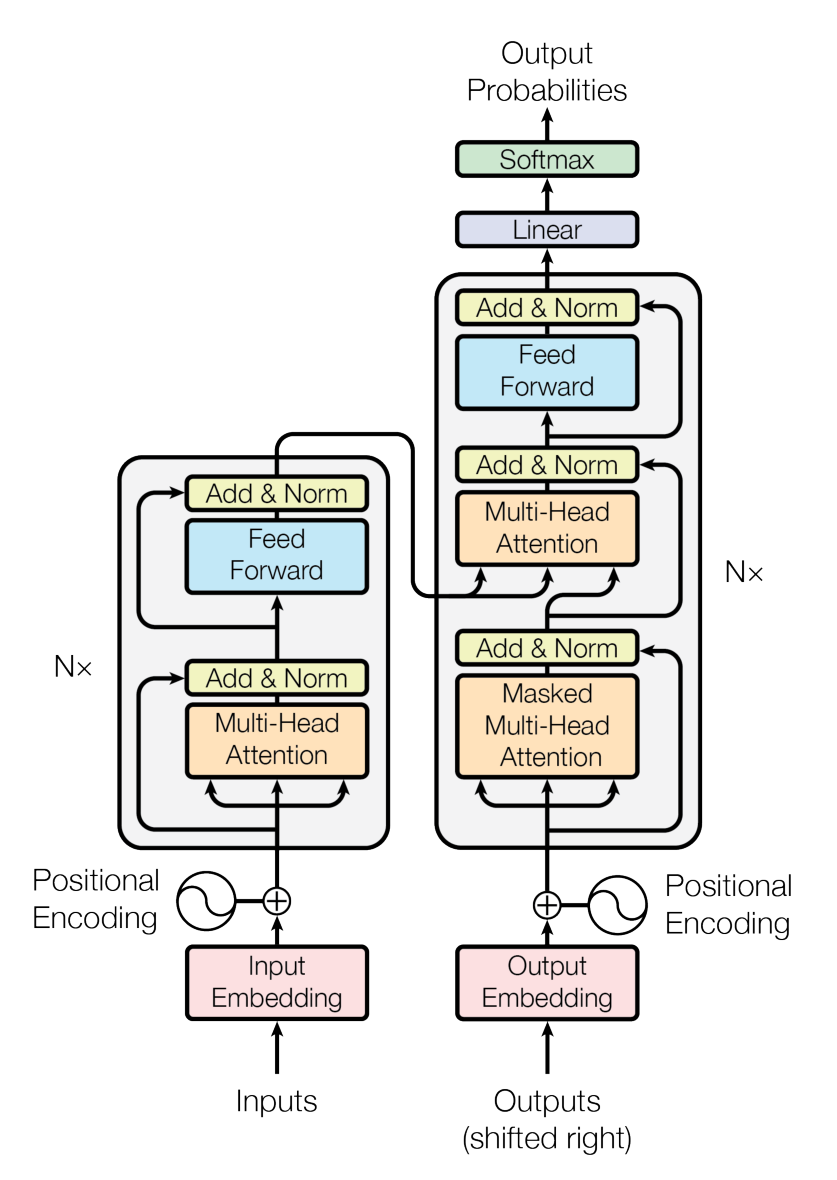
\includegraphics[width=0.23\textwidth]{transformer-architecture.png}
    \label{transformer-architecture}
  \end{figure}
  \begin{center}%
    \tiny Архитектура Transformer из статьи «Attention is all you need»
  \end{center}
\end{frame}


\begin{frame}[fragile]{Механизм внимания}%
  Механизм внимания может быть представлен формулой:
  \begin{equation}\label{scaled-dot-product-attention}%
    \operatorname{Attention}(Q, K, V) = \underbrace{
      \operatorname{softmax}\left(
        \frac{QK^T}{\sqrt{d_k}}
      \right)
    }_{\text{scores}}
    V,
  \end{equation}
  где
  \begin{itemize}%
    \item scores «оценивают» важность элементов (там лежат значения от 0 до 1);
    \item $Q$ (Query), $K$ (Key), $V$ (Value) "--- матрицы входных элементов;
    \item $d_k$ "--- нижняя размерность одной из этих матриц (длина части embedding'а).
  \end{itemize}
\end{frame}


\begin{frame}[fragile]{Positional encoding}%
  Так как в Transformer'е нет ни рекурренции (recurrence), ни свёртки, нам нужно что-то, что будет использовать порядок элементов в последовательности (positional encoding):
  \begin{equation}\label{positional-encoding}%
    PE(p, 2i) = \sin\left( \frac{p}{10\,000^{2i / d_{\text{model}}}} \right),
  \end{equation}
  \begin{equation}\label{positional-encoding-2}%
    PE(p, 2i + 1) = \cos\left( \frac{p}{10\,000^{(2i + 1) / d_{\text{model}}}} \right),
  \end{equation}
  где
  \begin{itemize}%
    \item $p$ (position) "--- позиция,
    \item $i$ (dimension) "--- размер предложения.
  \end{itemize}
\end{frame}

  %!TeX root = ../SimplifyJapanese.tex
\begin{frame}[fragile]{Архитектура системы}%
  Система состоит из:
  \begin{enumerate}[1.]%
    \item клиентского приложения \notImportant{(TypeScript + Lit)},
    \item сервера \notImportant{(Python + Falcon + MeCab)},
    \item модели ИНС \notImportant{(Python + PyTorch + Spacy + HuggingFace)}.
  \end{enumerate}
\end{frame}


\begin{frame}[fragile]{Корпус SNOW}%
  Маруяма~Т. и Ямамото~К. вручную составили корпус из 85\,000 предложений с их упрощёнными вариантами.

  Словарь упрощённых предложений в корпусе составляет лишь 2\,000 слов.
  
  Корпус состоит из 2-х частей:
  \begin{enumerate}[1.]%
    \item SNOW 15: 50\,000 предложений (только обучение),
    \item SNOW 23: 35\,000 предложений (33\,000/1\,000/1\,000 "--- train/valid/test).
  \end{enumerate}
\end{frame}


\begin{frame}[fragile]{Пользовательское приложение}%
  \begin{figure}[H]%
    \centering
    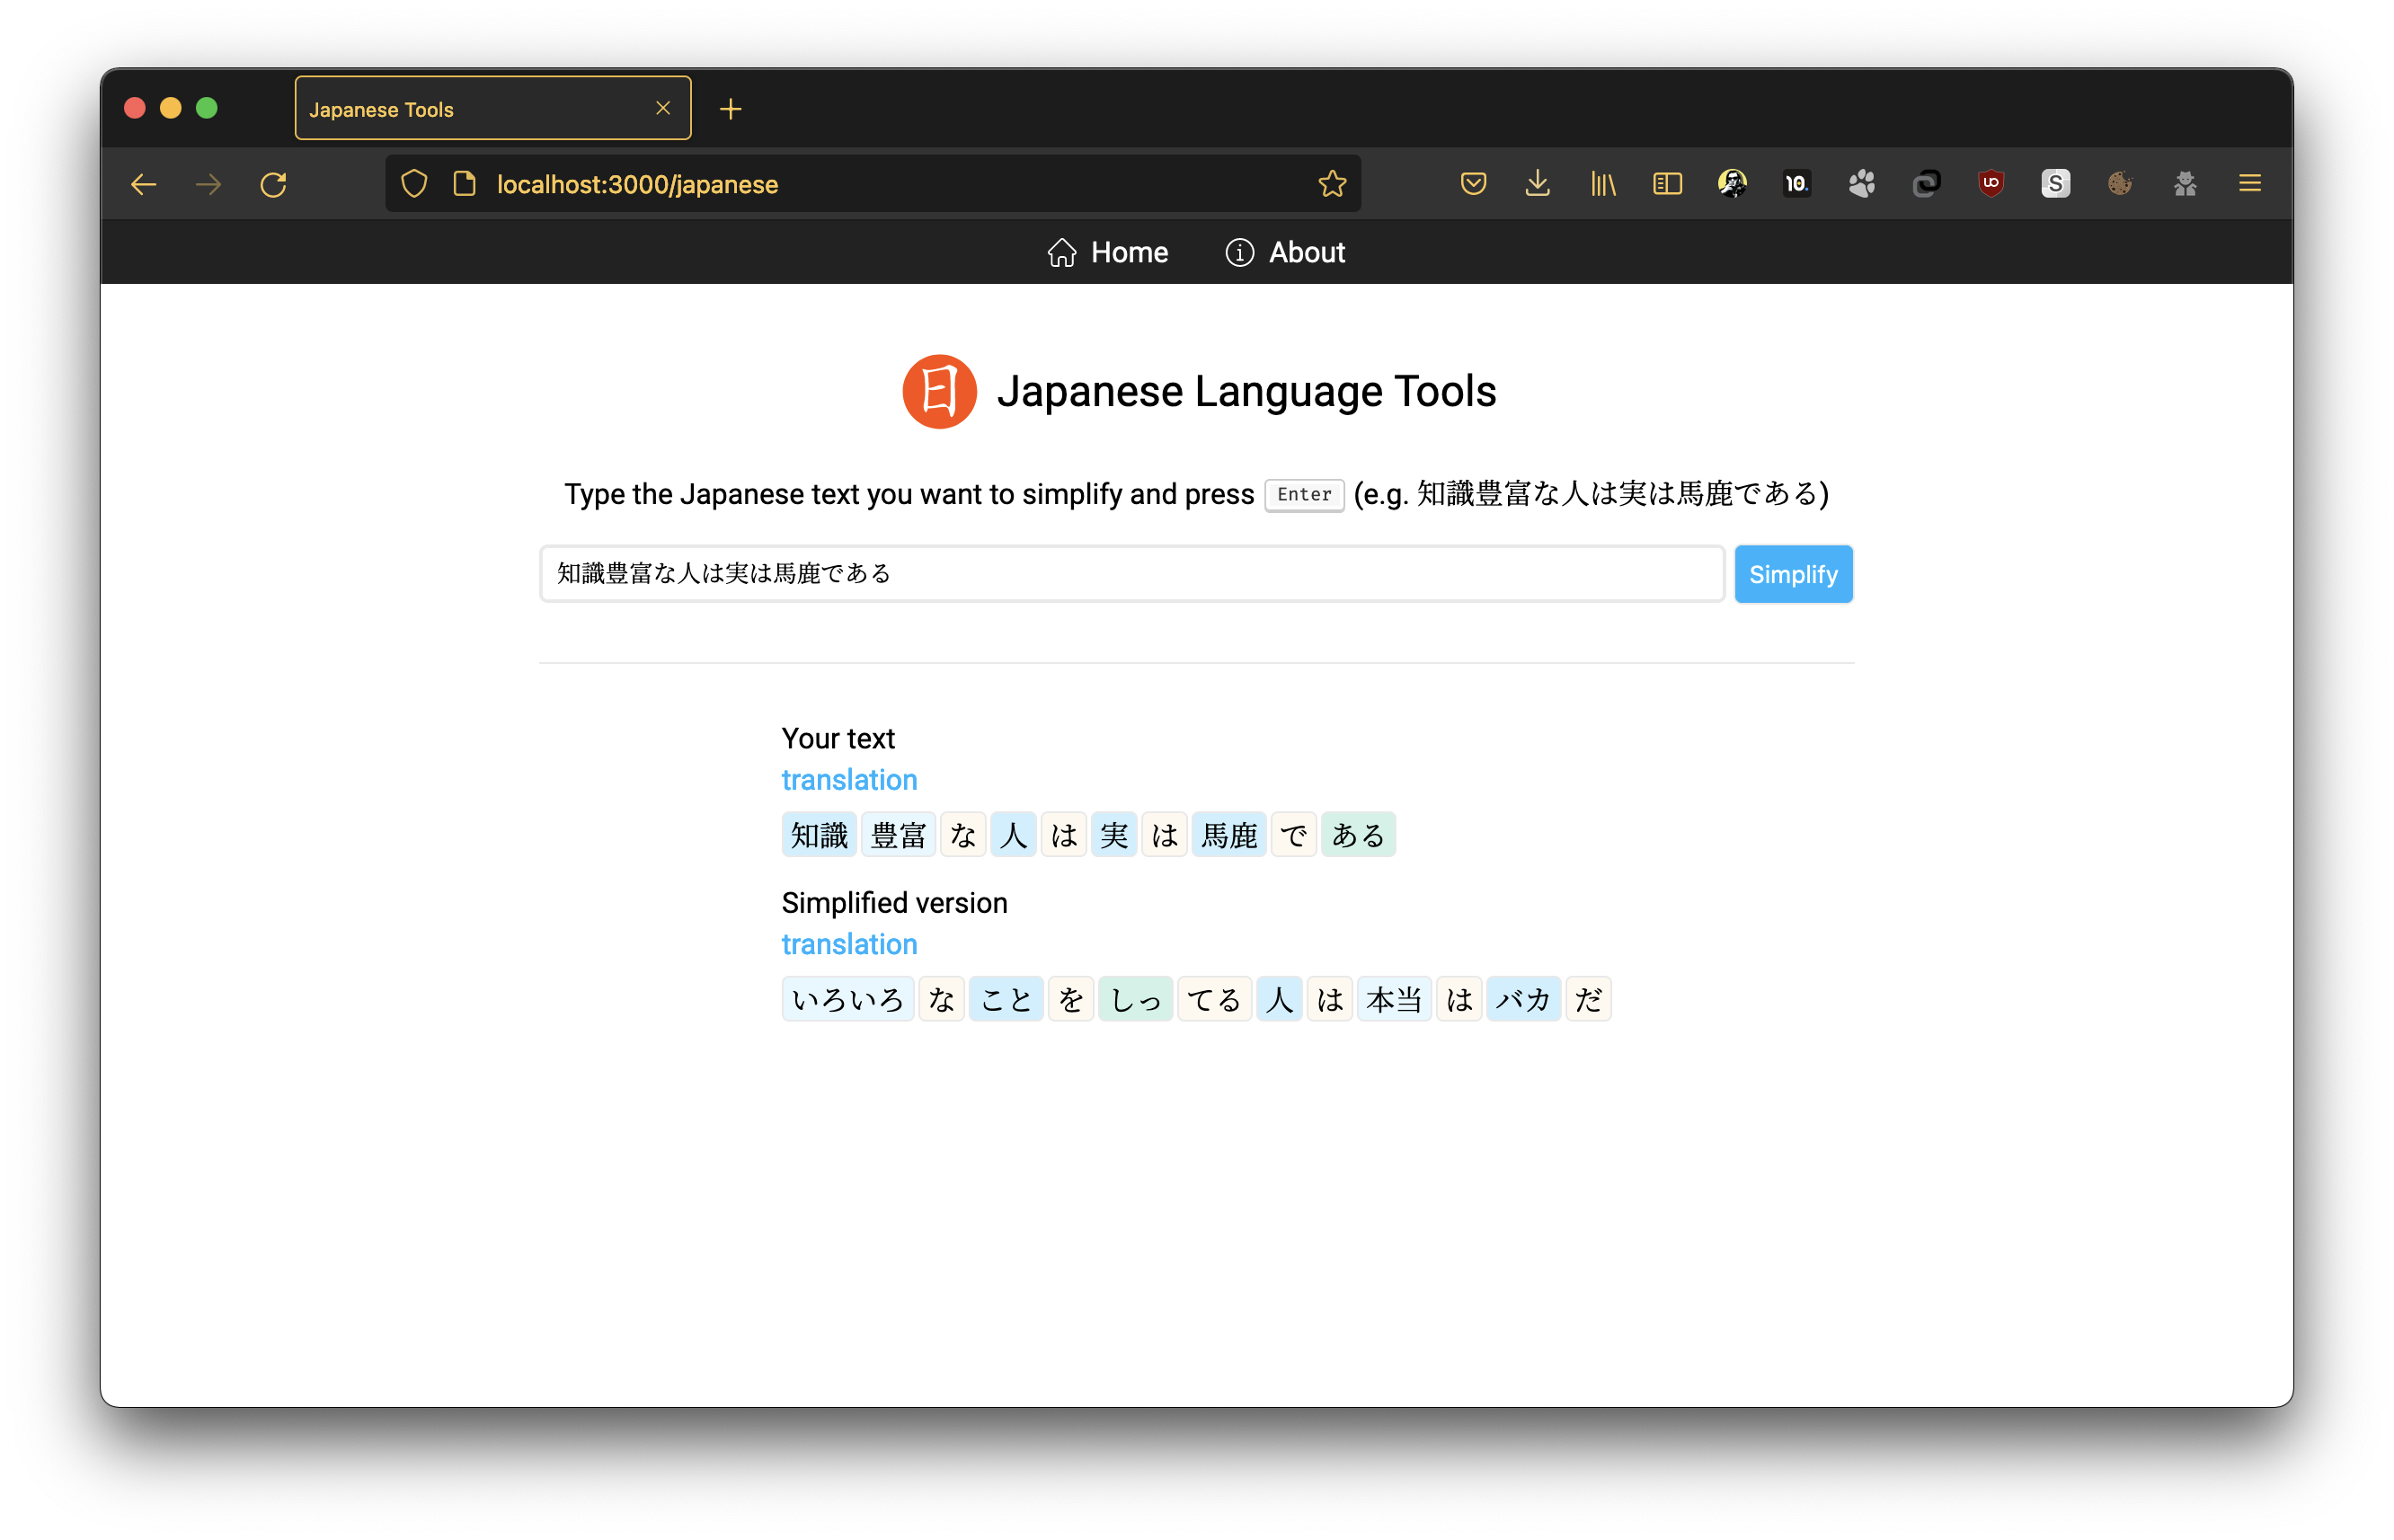
\includegraphics[width=0.6\textwidth]{app.png}
    \label{app-screen}
  \end{figure}
\end{frame}


\begin{frame}[fragile]{Проблемы реализованной системы}%
  Обученная модель обладает следующими недостатками:
  \begin{itemize}%
    \item плохо справляется с большими предложениями,
    \item имеет относительно небольшой «словарный запас».
  \end{itemize}

  Решение "--- предобучить \notImportant{(pretrain)} модель на неразмеченном корпусе и дообучить \notImportant{(fine-tune)} на корпусе SNOW:
  \begin{itemize}%
    \item Pretrained Transformer "--- предобучение всей модели,
    \item Pretrained Encoder "--- предобучение лишь encoder'а.
  \end{itemize}
\end{frame}

  %!TeX root = ../SimplifyJapanese.tex
\begin{frame}[fragile]{Метрики}%
  Метрики BLEU и SARI обученных моделей:
  \begin{table}[H]
    \centering\small
    \label{metrics}
      \begin{tabular}{|l|l|l|}
        \hline
        \textbf{Модель} & \textbf{BLEU} & \textbf{SARI} \\ \hline
        Transformer & 46{,}98 & 64{,}57 \\ \hline
        Pretrained Transformer & \textbf{51{,}12} & \textbf{67{,}89} \\ \hline
        Pretrained Encoder & 48{,}22 & 65{,}67 \\ \hline
      \end{tabular}
      \normalsize
  \end{table}
  Сравнение гистограмм метрик BLEU и SARI ({\color{mathematicaYellow}Transformer} / {\color{mathematicaBlue}Pretrained Transformer}):
  \begin{figure}[H]%
    \centering%
    \label{metrics-comparison}
    % \begin{subfigure}[H]{0.45\textwidth}
    %   \label{bleu-part}
      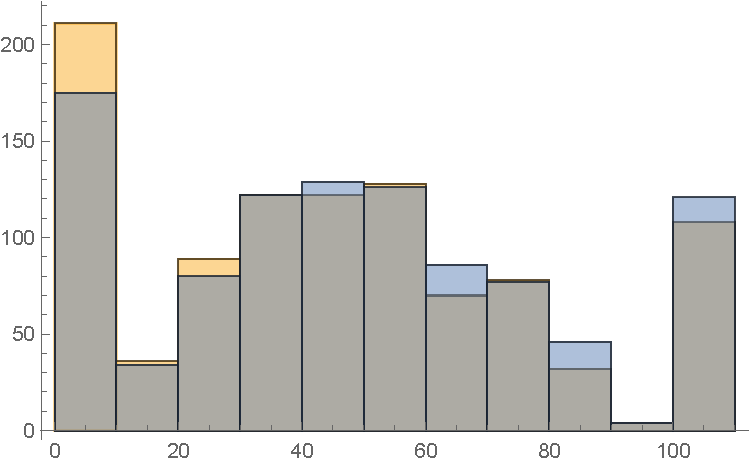
\includegraphics[width=0.3\textwidth]{bleu-comparison.pdf}
    %   \caption{Метрики BLEU}
    % \end{subfigure}
    % \begin{subfigure}[H]{0.45\textwidth}
      % \label{sari-part}
      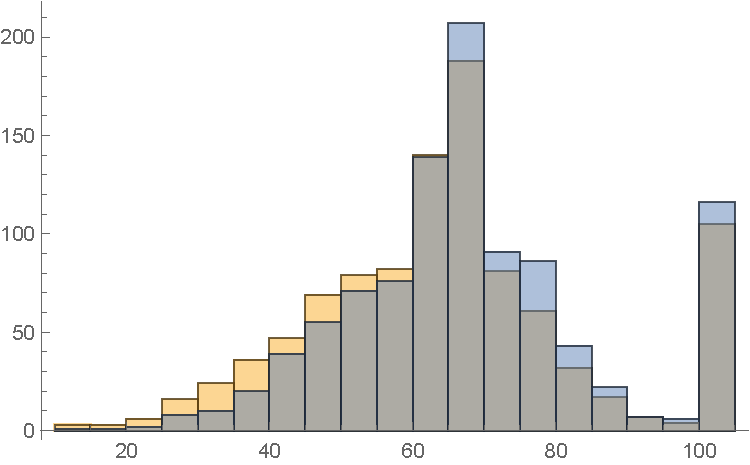
\includegraphics[width=0.3\textwidth]{sari-comparison.pdf}
    %   \caption{Метрики SARI}
    % \end{subfigure}
  \end{figure}%
\end{frame}


\begin{frame}[fragile]{Пример упрощения №1}%
  \sourceSentence{\jpExample{彼は怒りに我を忘れた}{он забылся в гневе}}

  \transformerSample{\jpExample{彼は怒っているのに自分の意見を忘れた}{он хоть и разозлился, но забыл своё мнение}}

  \pretrainedTransformerSample{\jpExample{彼は怒っていることに自分を忘れた}{он забылся, из-за того что разозлился}}

  \notImportant{Интересный момент:} «我» $\to$ «自分», "--- и то, и другое на русском просто «я», но на японском разные оттенки.
\end{frame}


\begin{frame}[fragile]{Пример упрощения №2}%
  \sourceSentence{\jpExample{入場料はただだった}{вход был бесплатным}}

  \transformerSample{\jpExample{入るためのお金はただなかった}{деньги для входа не были бесплатными}}

  \pretrainedTransformerSample{\jpExample{入るためのお金は0円だった}{денег для входа нужно было 0 йен}}

  Здесь происходит замена сложного слова из кандзи (入場料) на простую фразу (入るためのお金).
\end{frame}


\begin{frame}[fragile]{Пример упрощения №3}%
  \sourceSentence{\jpExample{そのスキャンダルはやがてみんなに知れ渡るだろう}{об этом скандале, вероятно, скоро узнают все}}

  \transformerSample{\jpExample{その事件を守る事件はやがてみんなに知られるだろう}{скоро об этом событии, защищающем событие, вероятно, узнают все}}

  \pretrainedTransformerSample{\jpExample{その悪い話はやがてみんなに知られるだろう}{об этой нехорошей истории скоро, вероятно, все узнают}}

  \notImportant{Интересный момент:} в корпусе представлен менее удачный вариант упрощения данного предложения. \\
  その悪い、知られたくないことは、やがてみんなに報告されるだろう \\ 
  "--- Об этом нехорошем деле, о котором никто не хочет знать, скоро всем доложат.
\end{frame}

  %!TeX root = ../Asq.tex
\begin{frame}{Заключение}%
  \begin{itemize}%
    \item Была изучена предметная область,
    \item были исследованы методы анализа и формализации русского языка,
    \item была разработана система трансляции запросов на русском языке в SQL-код,
    \item разработанная система была протестирована на запросах различной сложности.
  \end{itemize}
\end{frame}

\end{document}

% Добавить цель в выводах
% Слайды wide
